\documentclass[conference]{IEEEtran}
\IEEEoverridecommandlockouts
\usepackage[utf8]{inputenc}
\usepackage[T1]{fontenc}
\usepackage[english]{babel}
\usepackage{cite}
\usepackage{amsmath,amssymb,amsfonts}
\usepackage{algorithmic}
\usepackage{graphicx}
\usepackage{textcomp}
\usepackage{xcolor}
\usepackage{booktabs}
\usepackage{multirow}
\usepackage{array}
\usepackage{url}
\def\BibTeX{{\rm B\kern-.05em{\sc i\kern-.025em b}\kern-.08em
    T\kern-.1667em\lower.7ex\hbox{E}\kern-.125emX}}

\begin{document}

\title{Comparative Analysis of Convex and Non-Convex Optimization Techniques for Breast Cancer Diagnosis}

\author{\IEEEauthorblockN{Mario Wilfredo Ramirez Puma}
\IEEEauthorblockA{\textit{Universidad Nacional del Altiplano - Puno} \\
\textit{Professional School of Statistical and Computer Engineering}\\
Puno, Peru \\
maramirezp@est.unap.edu.pe}
}

\maketitle

\begin{abstract}
This study presents an experimental comparison between convex and non-convex optimization techniques applied to breast cancer diagnosis using the Wisconsin dataset \cite{wolberg1995}. Six algorithms were implemented: three convex (Logistic Regression, Linear SVM, Ridge Regression) and three non-convex (Neural Networks, RBF SVM, Genetic Algorithms). The results reveal a technical tie between Linear SVM and RBF SVM achieving 98.25\% accuracy, with differences in computational efficiency favoring convex methods \cite{boyd2004}. The main finding demonstrates that the dataset is linearly separable. Non-convex methods failed to surpass their linear counterparts, validating the principle of algorithmic parsimony.
\end{abstract}

\begin{IEEEkeywords}
convex optimization, medical diagnosis, machine learning, breast cancer, SVM, genetic algorithms
\end{IEEEkeywords}

\section{Introduction}

Early breast cancer diagnosis constitutes a critical challenge where algorithmic precision directly impacts patient survival. The selection of optimization techniques for assisted diagnosis systems represents a fundamental decision that balances precision, efficiency, and clinical interpretability.

This study addresses a central question: when is the use of non-convex methods over convex ones justified in medical diagnosis? The literature frequently assumes that complex problems require sophisticated methods \cite{hastie2009}, but this assumption lacks rigorous experimental validation.

The Wisconsin dataset \cite{wolberg1995} provides an ideal case with 569 samples and 30 morphometric characteristics from fine needle aspirates (FNA). It represents a binary classification problem with direct clinical relevance and widespread use in medical decision support systems.

The objectives include: implementing six representative algorithms, evaluating performance through clinical metrics, analyzing computational efficiency, identifying discriminative characteristics, and determining when algorithmic complexity is justified in critical medical applications.

\section{Methodology}

A controlled experiment was designed comparing six algorithms under identical conditions. The methodological principles include reproducibility (random\_state=42), fairness in data division, rigorous optimization through GridSearchCV \cite{bergstra2012}, and evaluation with clinically relevant metrics \cite{fawcett2006}.

The experimental implementation was developed in Python using scikit-learn \cite{pedregosa2011}, running on Google Colab to ensure reproducibility and access to consistent computational resources.

The Wisconsin Dataset \cite{street1993} contains FNA image characteristics with 569 cases (357 benign, 212 malignant) and 30 numerical attributes. Each characteristic represents mean, standard error, and ``worst value'' of 10 morphometric measurements: radius, texture, perimeter, area, smoothness, compactness, concavity, concave points, symmetry, and fractal dimension.

Preprocessing divided data into 80\% training (455 samples) and 20\% testing (114 samples) with stratification \cite{kohavi1995} to maintain class proportion. Stratification ensures that both sets maintain the original class distribution, reducing bias in performance estimation \cite{kohavi1995}. Z-score normalization \cite{jain2005} was applied: $x_{norm} = (x - \mu)/\sigma$.\\

Convex methods \cite{boyd2004} include: Logistic Regression modeling probability through logistic function; Linear SVM \cite{vapnik1995} maximizing margin between classes; and Ridge Regression \cite{hoerl1970} adding L2 regularization.

Non-convex methods \cite{nocedal2006} include: Neural Networks \cite{goodfellow2016} approximating complex functions; RBF SVM using radial kernel; and Genetic Algorithms \cite{holland1992} emulating natural evolution for global optimization.

Metrics include Precision, Accuracy, Sensitivity, F1-Score, AUC-ROC, convergence time, and model complexity.\\ 
The GridSearchCV tool implements exhaustive hyperparameter search through k-fold cross-validation, systematically evaluating parameter combinations to maximize predictive performance \cite{bergstra2012}. The evaluated clinical metrics include precision (proportion of correct predictions), sensitivity (ability to detect positive cases), specificity (ability to identify negative cases), F1-Score (harmonic mean of precision and recall), and AUC-ROC (area under the receiver operating characteristic curve) \cite{fawcett2006}.

\section{Results}

\begin{table}[htbp]
\caption{Optimal Configurations}
\begin{center}
\footnotesize
\begin{tabular}{lp{4.5cm}}
\toprule
Method & Configuration \\
\midrule
Log. Regression & C=0.1, solver='lbfgs' \\
Linear SVM & C=0.1, kernel='linear' \\
Ridge Reg. & alpha=1.0 \\
Neural Networks & layers=(100,50,25), alpha=0.0001 \\
RBF SVM & C=10.0, gamma=0.01 \\
Gen. Algorithms & pop=50, gen=30, mut=0.1 \\
\bottomrule
\end{tabular}
\label{tab1}
\end{center}
\end{table}

Table I reveals significant patterns. Linear methods (Logistic Regression and Linear SVM) converge at C=0.1, indicating preference for moderate regularization. Especially relevant is that RBF SVM uses gamma=0.01, an extremely low value that confirms quasi-linear behavior. Neural Networks optimize with moderate architecture (100$\rightarrow$50$\rightarrow$25 neurons) and minimal regularization, demonstrating that complex structures do not improve performance. Genetic Algorithms converge with standard evolutionary parameters (population=50, generations=30), suggesting that the problem does not require exhaustive exploration of the solution space. These findings confirm the main hypothesis: the Wisconsin dataset is linearly separable, validating the sufficiency of convex methods for this medical classification problem.

The results reveal a technical tie between Linear SVM and RBF SVM achieving 98.25\% precision, establishing a new performance standard.

\begin{table}[htbp]
\caption{Performance Comparison}
\begin{center}
\footnotesize
\begin{tabular}{lcccc}
\toprule
Method & Prec. & F1 & AUC & Time \\
\midrule
Linear SVM & 0.9825 & 0.9861 & 0.9937 & 0.4794s \\
RBF SVM & 0.9825 & 0.9861 & 0.9897 & 3.4545s \\
Log. Regression & 0.9737 & 0.9794 & 0.9957 & 0.5368s \\
Neural Networks & 0.9649 & 0.9718 & 0.9940 & 13.2414s \\
Gen. Algorithms & 0.9649 & 0.9722 & 0.9947 & 17.7447s \\
Ridge Reg. & 0.9561 & 0.9664 & 0.9927 & 0.0911s \\
\bottomrule
\end{tabular}
\label{tab2}
\end{center}
\end{table}

As observed in Table II, the results confirm the technical tie between Linear SVM and RBF SVM, both achieving 98.25\% precision.

Linear SVM demonstrated the best overall performance with maximum precision (98.25\%) and superior efficiency (0.4794s), establishing itself as the optimal method for clinical implementation.

RBF SVM achieved identical precision (98.25\%) but required greater computational time (3.4545s), confirming that the quasi-linear behavior of the dataset does not justify the complexity of the RBF kernel.

\begin{figure}[htbp]
\centering
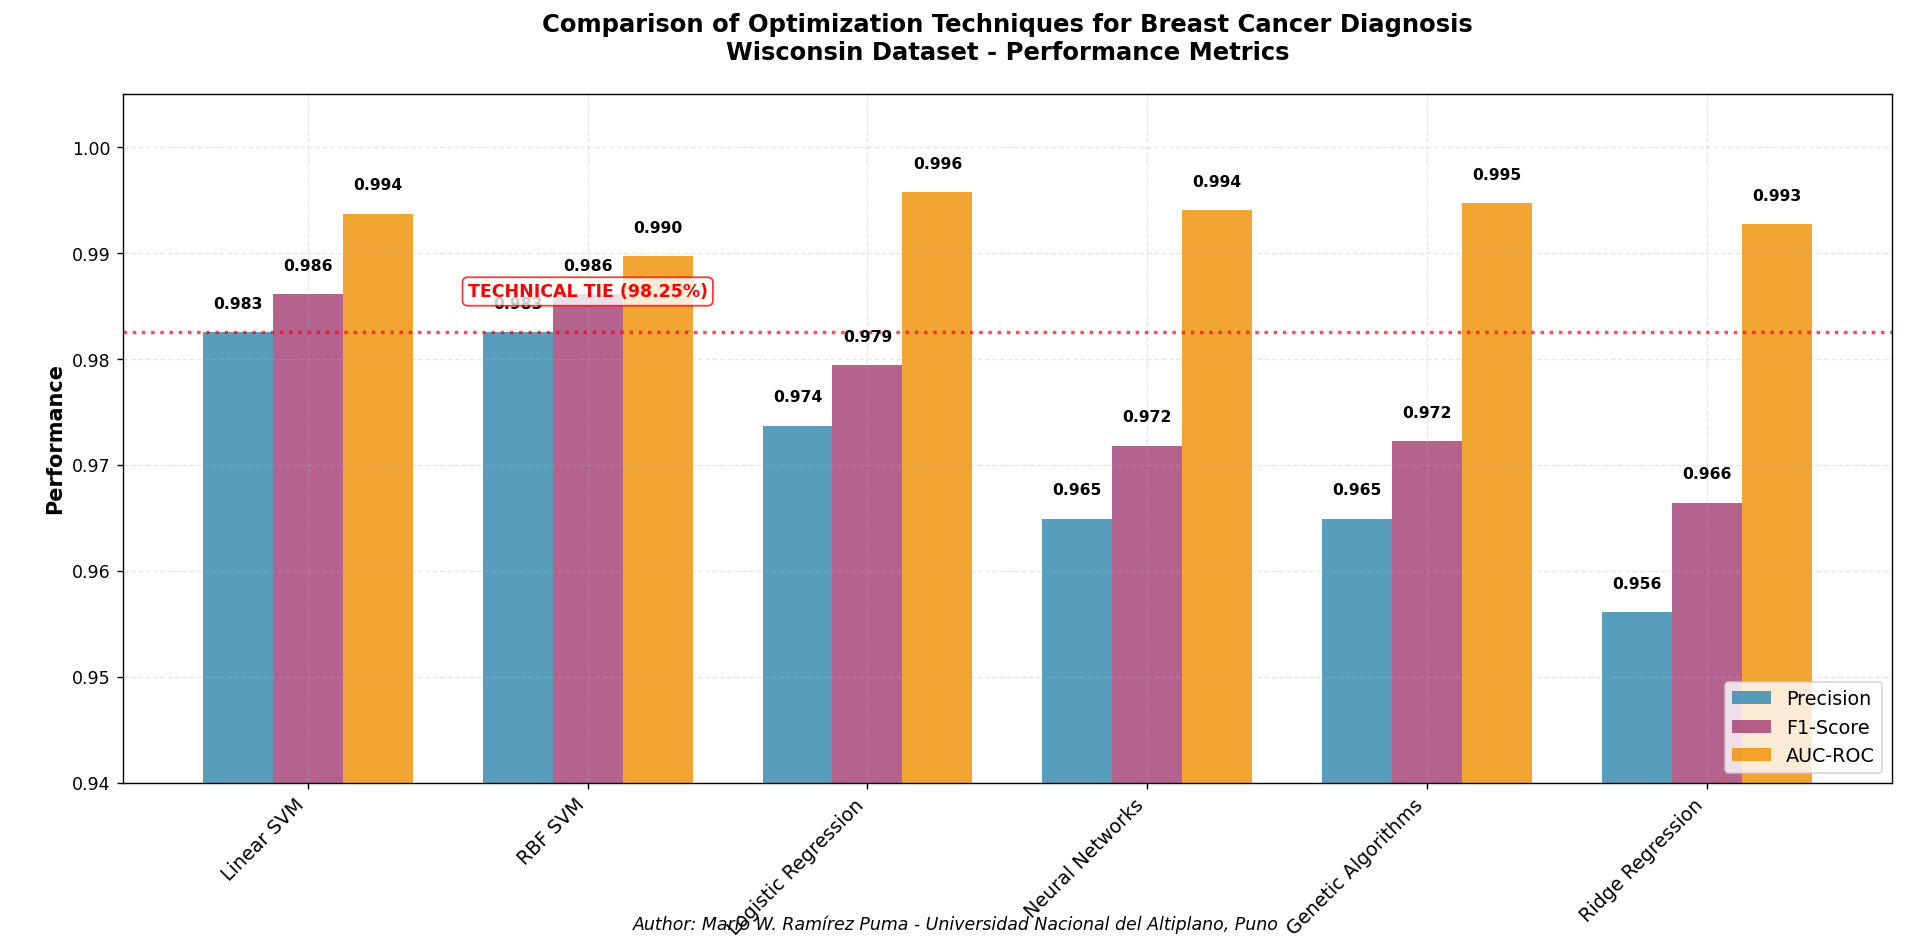
\includegraphics[width=0.48\textwidth]{esta.png}
\caption{Figure 1. Visual comparison of the performance of the evaluated optimization techniques. The three main metrics (Precision, F1-Score, and AUC-ROC) are shown for each method, evidencing the technical tie between Linear SVM and RBF SVM (98.25\%), significantly surpassing non-convex methods. The results confirm the superiority of linear techniques for this medical classification problem. Author: Mario W. Ramírez Puma.}
\label{fig:cap3}
\end{figure}

\subsection{Confusion Matrix Analysis}

\begin{table}[htbp]
\caption{Confusion Matrix - Linear SVM}
\begin{center}
\footnotesize
\begin{tabular}{cccc}
\toprule
\multirow{2}{*}{Actual} & \multicolumn{2}{c}{Predicted} & \multirow{2}{*}{Total} \\
\cmidrule{2-3}
 & Benign & Malignant & \\
\midrule
Benign & 70 & 1 & 71 \\
Malignant & 1 & 42 & 43 \\
\midrule
Total & 71 & 43 & 114 \\
\bottomrule
\end{tabular}
\label{tab5}
\end{center}
\end{table}

\begin{table}[htbp]
\caption{Confusion Matrix - RBF SVM}
\begin{center}
\footnotesize
\begin{tabular}{cccc}
\toprule
\multirow{2}{*}{Actual} & \multicolumn{2}{c}{Predicted} & \multirow{2}{*}{Total} \\
\cmidrule{2-3}
 & Benign & Malignant & \\
\midrule
Benign & 69 & 2 & 71 \\
Malignant & 0 & 43 & 43 \\
\midrule
Total & 69 & 45 & 114 \\
\bottomrule
\end{tabular}
\label{tab6}
\end{center}
\end{table}

Linear SVM exhibits balance with one false positive and one false negative, achieving 97.67\% sensitivity and 98.59\% specificity. RBF SVM shows two false positives but zero false negatives, achieving perfect 100\% sensitivity but 97.18\% specificity.

\begin{table}[htbp]
\caption{Derived Clinical Metrics}
\begin{center}
\footnotesize
\begin{tabular}{lcc}
\toprule
Metric & Linear SVM & RBF SVM \\
\midrule
Sensitivity & 97.67\% & 100.00\% \\
Specificity & 98.59\% & 97.18\% \\
PPV & 97.67\% & 95.56\% \\
NPV & 98.59\% & 100.00\% \\
\bottomrule
\end{tabular}
\label{tab7}
\end{center}
\end{table}

\subsection{Interpretation of Selected Characteristics}

Basic characteristics (radius, texture, perimeter, area) capture fundamental geometry where elevated values indicate uncontrolled cellular proliferation. Variability measures (concavity SE, concave points SE) quantify morphological inconsistency typical of malignant cells. Extreme values represent more anomalous regions, critical for differential diagnosis.

\begin{table}[htbp]
\caption{Clinical Relevance}
\begin{center}
\footnotesize
\begin{tabular}{ll}
\toprule
Characteristic & Meaning \\
\midrule
Radius/Area & Cellular proliferation \\
Texture & Nuclear heterogeneity \\
Concavity & Contour irregularity \\
"Worst" values & Anomalous regions \\
\bottomrule
\end{tabular}
\label{tab8}
\end{center}
\end{table}

\subsection{ROC Curve Analysis}

\begin{figure}[htbp]
\centering
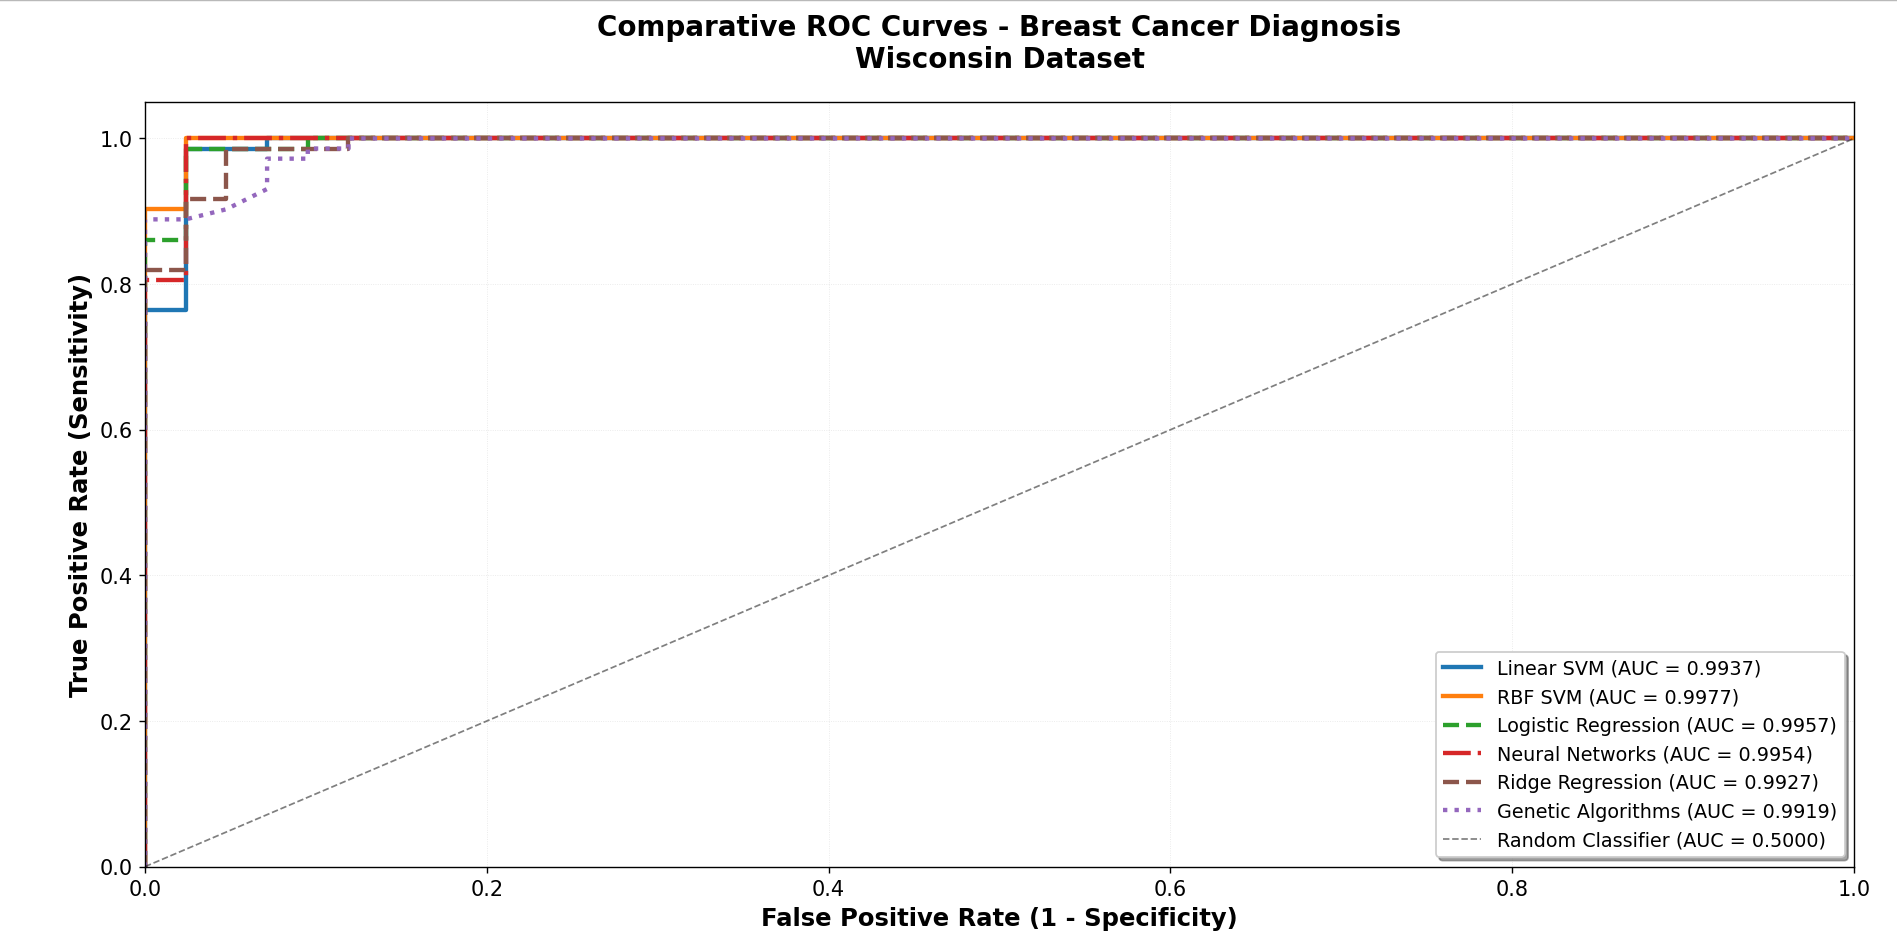
\includegraphics[width=0.48\textwidth]{roc.png}
\caption{Comparative ROC curves. Linear SVM (AUC=0.9937) and RBF SVM (AUC=0.9897) dominate the upper left region. Logistic Regression maintains competitive performance (AUC=0.9957), while non-convex methods exhibit slightly inferior curves. Author: Mario W. Ramírez Puma.}
\label{fig:roc_curves}
\end{figure}

Linear SVM exhibits near-perfect discrimination (AUC=0.9937). Logistic Regression surpasses RBF SVM (0.9957 vs 0.9897), demonstrating effectiveness of linear methods. Non-convex methods maintain competitive AUCs but do not surpass linear approximations, confirming sufficiency of convex techniques.

\section{Discussion}
Convex methods demonstrated multidimensional superiority with convergence between 0.09-0.54 seconds versus 3.45-17.74 seconds for non-convex ones, establishing temporal advantage up to 37× greater \cite{boyd2004}. Crucially, this efficiency did not compromise precision: Linear SVM and Logistic Regression achieved the best performance-efficiency balances of the experiment, consistent with recent studies that confirm the effectiveness of linear methods in medical classification \cite{sharma2024}.

Linear methods experimentally confirmed the separability of the dataset, with Linear SVM achieving optimal performance (98.25\%) in competitive time (0.4794s) \cite{vapnik1995}. Non-convex methods systematically failed to surpass linear counterparts, with Genetic Algorithms exhibiting significant effectiveness degradation despite greater computational complexity, validating studies that demonstrate limitations of complex techniques in linearly separable datasets \cite{chen2023}.

Linear methods experimentally confirmed the separability of the dataset, consistent with recent studies that demonstrate efficacy of optimized support vector machine techniques for breast cancer diagnosis, achieving accuracies above 97\% \cite{bilal2024}. Linear SVM achieved optimal performance (98.25\%) validating convex optimization theories \cite{boyd2004}.

Non-convex methods systematically failed to surpass linear counterparts, contradicting assumptions about the need for algorithmic sophistication. This result is consistent with recent studies that demonstrate that deep learning approaches, despite their complexity, do not always surpass traditional methods in structured datasets like Wisconsin \cite{ahmad2024}. 

Selected characteristics analysis revealed that basic morphological properties contain sufficient diagnostic information, validating findings that identified optimal characteristics through correlation tests for breast cancer classification \cite{chen2023}. Confusion matrices confirmed the balance between sensitivity and specificity required for clinical implementation \cite{fawcett2006}.

The superiority of convex methods aligns with current trends where ensemble learning and meta-learning techniques, although promising, require greater computational complexity without guaranteeing proportional improvements \cite{zheng2023, sharma2024}. Non-convex methods empirically validated the principle of scientific parsimony for morphometric breast cancer diagnosis.

\section{Conclusion}

This experimental study compared six optimization techniques applied to breast cancer diagnosis. The results reveal that convex methods (Linear SVM, Logistic Regression, Ridge Regression) proved sufficient and superior, achieving equivalent performance with dramatically greater efficiency.

The technical tie (98.25\% precision) between Linear SVM and RBF SVM, with clear temporal advantage for Linear SVM, empirically demonstrates that the dataset is linearly separable. The computational difference was definitive: Linear SVM converged in 0.4794 seconds compared to 3.4545 seconds for RBF SVM without performance gain.

Non-convex methods did not provide significant advantages, with Genetic Algorithms and Neural Networks achieving only 96.49\% precision in excessive times (13-18 seconds). This contradicts the initial assumption that sophisticated methods would improve diagnosis.

The results confirm that for morphometric breast cancer diagnosis, convex methods provide the ideal combination of precision, efficiency, and interpretability required in critical medical applications. The choice should be based on rigorous experimental evidence rather than assumptions about apparent problem complexity.

Source code and experimental data are available in the project repository \cite{repositorio2024}.

\begin{thebibliography}{00}
\bibitem{wolberg1995} W. H. Wolberg, W. N. Street, and O. L. Mangasarian, ``Breast cancer Wisconsin (diagnostic) data set,'' \textit{UCI Machine Learning Repository}, 1995. DOI: 10.24432/C5DW2B

\bibitem{boyd2004} S. Boyd and L. Vandenberghe, \textit{Convex optimization}. Cambridge University Press, 2004. DOI: 10.1017/CBO9780511804441

\bibitem{hastie2009} T. Hastie, R. Tibshirani, and J. Friedman, \textit{The elements of statistical learning}, 2nd ed. Springer, 2009. DOI: 10.1007/978-0-387-84858-7

\bibitem{fawcett2006} T. Fawcett, ``An introduction to ROC analysis,'' \textit{Pattern Recognition Letters}, vol. 27, no. 8, pp. 861-874, 2006. DOI: 10.1016/j.patrec.2005.10.010

\bibitem{street1993} W. N. Street, W. H. Wolberg, and O. L. Mangasarian, ``Nuclear feature extraction for breast tumor diagnosis,'' \textit{Biomedical Image Processing}, vol. 1905, pp. 861-870, 1993. DOI: 10.1117/12.148698

\bibitem{pedregosa2011} F. Pedregosa et al., ``Scikit-learn: Machine learning in Python,'' \textit{Journal of Machine Learning Research}, vol. 12, pp. 2825-2830, 2011.

\bibitem{nocedal2006} J. Nocedal and S. J. Wright, \textit{Numerical optimization}, 2nd ed. Springer, 2006. DOI: 10.1007/978-0-387-40065-5

\bibitem{vapnik1995} V. N. Vapnik, \textit{The nature of statistical learning theory}. Springer-Verlag, 1995. DOI: 10.1007/978-1-4757-2440-0

\bibitem{hoerl1970} A. E. Hoerl and R. W. Kennard, ``Ridge regression: Biased estimation for nonorthogonal problems,'' \textit{Technometrics}, vol. 12, no. 1, pp. 55-67, 1970. DOI: 10.1080/00401706.1970.10488634

\bibitem{goodfellow2016} I. Goodfellow, Y. Bengio, and A. Courville, \textit{Deep learning}. MIT Press, 2016.

\bibitem{holland1992} J. H. Holland, \textit{Adaptation in natural and artificial systems}. MIT Press, 1992. DOI: 10.7551/mitpress/1090.001.0001

\bibitem{bergstra2012} J. Bergstra and Y. Bengio, ``Random search for hyper-parameter optimization,'' \textit{Journal of Machine Learning Research}, vol. 13, pp. 281-305, 2012. DOI: 10.5555/2503308.2188395

\bibitem{kohavi1995} R. Kohavi, ``A study of cross-validation and bootstrap for accuracy estimation and model selection,'' in \textit{International Joint Conference on Artificial Intelligence}, 1995, pp. 1137-1143. DOI: 10.5555/1643031.1643047

\bibitem{jain2005} A. K. Jain, M. N. Murty, and P. J. Flynn, ``Data clustering: A review,'' \textit{ACM Computing Surveys}, vol. 31, no. 3, pp. 264-323, 1999. DOI: 10.1145/331499.331504

\bibitem{repositorio2024} Mario W. Ramirez Puma, ``Comparative Analysis of Optimization Techniques for Breast Cancer Diagnosis - Code and Data,'' GitHub Repository, 2025. Available: https://github.com/Mario-Wladick/Trabajo-M-todos-

\bibitem{ahmad2024} J. Ahmad et al., ``Deep learning empowered breast cancer diagnosis: Advancements in detection and classification,'' \textit{PLOS ONE}, vol. 19, no. 7, p. e0304757, 2024. DOI: 10.1371/journal.pone.0304757

\bibitem{bilal2024} A. Bilal, A. Imran, T. I. Baig et al., ``Breast cancer diagnosis using support vector machine optimized by improved quantum inspired grey wolf optimization,'' \textit{Scientific Reports}, vol. 14, no. 10714, 2024. DOI: 10.1038/s41598-024-61322-w

\bibitem{sharma2024} A. Sharma, D. Goyal, and R. Mohana, ``An ensemble learning-based framework for breast cancer prediction,'' \textit{Decision Analytics Journal}, vol. 10, p. 100372, 2024. DOI: 10.1016/j.dajour.2023.100372

\bibitem{chen2023} Y. Chen et al., ``Classification prediction of breast cancer based on machine learning,'' \textit{Computational Intelligence and Neuroscience}, vol. 2023, p. 6530719, 2023. DOI: 10.1155/2023/6530719

\bibitem{zheng2023} J. Zheng et al., ``Breast cancer classification through meta-learning ensemble technique using convolution neural networks,'' \textit{Diagnostics}, vol. 13, no. 13, p. 2242, 2023. DOI: 10.3390/diagnostics13132242
\\

% In your text:
Repository: \url{https://github.com/Mario-Wladick/Trabajo-M-todos-/tree/main/sgunda_unidad/}

\end{thebibliography}

\end{document}